\documentclass[a4paper,14pt]{article}
\usepackage{float}
\usepackage{extsizes}
\usepackage{amsmath}
\usepackage{amssymb}
\everymath{\displaystyle}
\usepackage{geometry}
\usepackage{fancyhdr}
\usepackage{multicol}
\usepackage{graphicx}
\usepackage[brazil]{babel}
\usepackage[shortlabels]{enumitem}
\usepackage{cancel}
\usepackage{textcomp}
\columnsep=2cm
\hoffset=0cm
\textwidth=8cm
\setlength{\columnseprule}{.1pt}
\setlength{\columnsep}{2cm}
\renewcommand{\headrulewidth}{0pt}
\geometry{top=1in, bottom=1in, left=0.7in, right=0.5in}

\pagestyle{fancy}
\fancyhf{}
\fancyfoot[C]{\thepage}

\begin{document}
	
	\noindent\textbf{8FMA73 - Matemática} 
	
	\begin{center}Relações cujos gráficos são retas (Versão estudante)
	\end{center}
	
	\noindent\textbf{Nome:} \underline{\hspace{10cm}}
	\noindent\textbf{Data:} \underline{\hspace{4cm}}
	
	%\section*{Questões de Matemática}
	
	
    \begin{multicols}{2}
    	\noindent Toda relação da forma $Ax + By + C = 0$, com $A$, $B$ e $C$ reais, sendo $A$ e $B$ não ambos nulos, tem como gráfico uma reta.
    	\noindent\textsubscript{~---------------------------------------------------------------------------}
		\begin{enumerate}
			\item Fazer os gráficos das relações:
			\begin{enumerate}[a)]
				\item $y = -x$ \\\\\\\\\\\\\\\\\\\\\\\\\\
				\item $y = -4$ \\\\\\\\\\\\\\\\\\\\\\\\\\
				\item $x - 2 = 0$ \\\\\\\\\\\\\\\\\\\\\\\\\\\\\\\\
				\item $y - 3x - 3 = 0$ \\\\\\\\\\\\\\\\\\\\\\\\\\\\\\\\
			\end{enumerate}
		    \item Determine uma relação entre $x$ e $y$ cujo gráfico seja uma reta que passa por:
		    \begin{enumerate}[a)]
		    	\item $(3; 2)$ e $(0; 0)$. \\\\\\\\\\\\\\\\\\\\\\\\
		    	\item $(-2; 1)$ e $(3; 0)$. \\\\\\\\\\\\\\\\\\\\\\\\
		    	\item $(4; 4)$ e $(-1; 1)$. \\\\\\\\\\\\\\\\\\
		    \end{enumerate}
	        \item Determine $a$, $a \in \mathbb{R}$, para que a relação $3y + ax + a^2 = 0$ tenha como gráfico a seguinte reta:
	        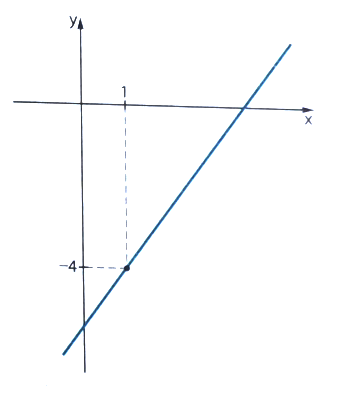
\includegraphics[width=1\linewidth]{imagens_8FMA73/imagem1} \\\\\\\\\\\\\\\\\\\\\\\\\\\\\\\\\\\\\\\\\\\\\\
	        \item Faça o gráfico das seguintes relações:
	        \begin{enumerate}[a)]
		        \item $
		        \begin{cases} 
		        	y = -x \\
		        	~~~~~\text{e} \\
		        	y = 3x + 2
		        \end{cases}$\\\\\\\\\\\\\\\\\\\\\\\\\\\\\\\\
	            \item $
	            \begin{cases} 
	            	y = -x \\
	            	~~~~~\text{ou} \\
	            	y = 3x + 2
	            \end{cases}$\\\\\\\\\\\\\\\\\\\\\\\\\\\\\\\\
            \end{enumerate}
            \item Fazer os gráficos das relações:
            \begin{enumerate}[a)]
            	\item $x + y = 0$ \\\\\\\\\\\\\\\\\\\\\\\\\\
            	\item $y = -2$ \\\\\\\\\\\\\\\\\\\\\\\\\\\\
            	\item $x - 1 = 0$ \\\\\\\\\\\\\\\\\\
            	\item $7x + 3y - 2 = 0$ \\\\\\\\\\\\\\\\\\\\\\\\
            \end{enumerate}
            \item Calcule a área do trapézio em destaque.\\
            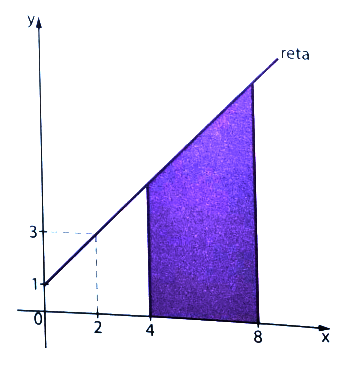
\includegraphics[width=1\linewidth]{imagens_8FMA73/imagem2} \\\\\\\\\\\\\\\\\\\\\\\\\\
            \item Qual a área do triângulo definido pelas retas $y = \frac{1}{3}x$, $y = \frac{2}{5}$ e $x = 0$?
        \end{enumerate}
    $~$ \\ $~$ \\ $~$ \\ $~$ \\ $~$ \\ $~$ \\ $~$ \\ $~$ \\ $~$ \\ $~$ \\ $~$ \\ $~$ \\ $~$ \\ $~$ \\ $~$ \\ $~$ \\ $~$ \\ $~$ \\ $~$ \\ $~$ \\ $~$ \\ $~$ \\ $~$ \\ $~$ \\ $~$ \\ $~$ \\ $~$ \\ $~$ \\ $~$ \\ $~$ \\ $~$ \\ $~$ \\ $~$ \\ $~$ \\ $~$ \\ $~$ \\ $~$ \\ 
    \end{multicols}
\end{document}